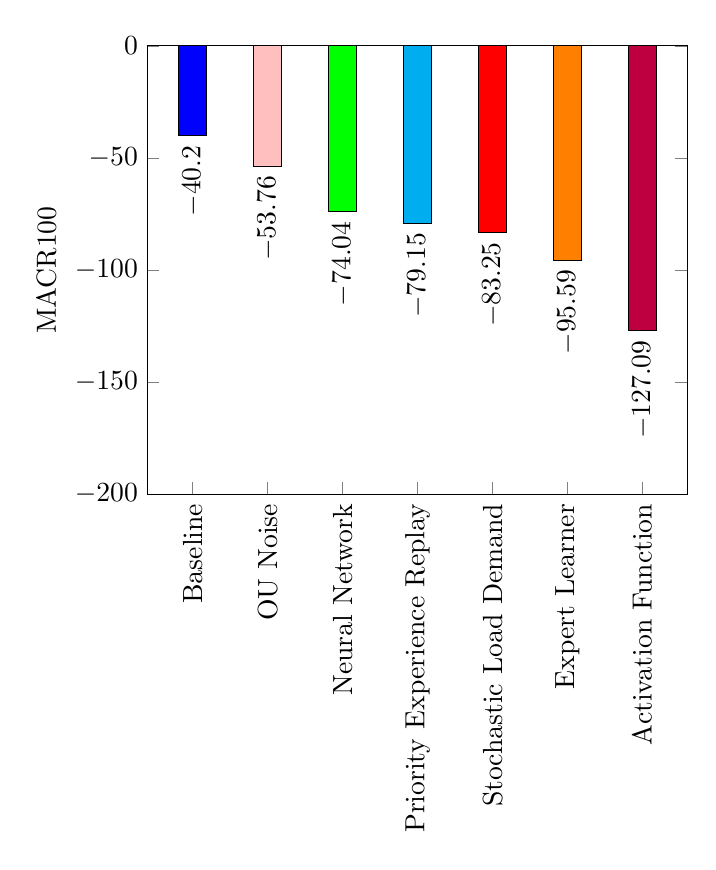
\begin{tikzpicture}
	\begin{axis}[
	    ylabel={MACR100},
	    symbolic x coords={Baseline,, OU Noise,, Neural Network,, Priority Experience Replay,, Stochastic Load Demand,, Expert Learner,, Activation Function},
	    xtick = {Baseline, Neural Network, Activation Function, OU Noise, Priority Experience Replay, Expert Learner, Stochastic Load Demand},
	    xticklabel style={rotate=90},
	    nodes near coords,
	    nodes near coords align={vertical},
	    every node near coord/.append style={rotate=90, anchor=east},
	    ymin=-200, ymax=0
	    ]
	\addplot [ybar, fill=blue] coordinates {(Baseline, -40.20)};
	\addplot [ybar, fill=green] coordinates {(Neural Network, -74.04)};
	\addplot [ybar, fill=purple] coordinates {(Activation Function, -127.09)};
	\addplot [ybar, fill=pink] coordinates {(OU Noise, -53.76)};
	\addplot [ybar, fill=cyan] coordinates {(Priority Experience Replay, -79.15)};
	\addplot [ybar, fill=orange] coordinates {(Expert Learner, -95.59)};
	\addplot [ybar, fill=red] coordinates {(Stochastic Load Demand, -83.25)};
	%\legend{Baseline, Neural Network, Activation Function, OU Noise, Priority Experience Replay, Expert Learner, Stochastic Load Demand};
	\end{axis}
\end{tikzpicture}